\section{Datastruktur}
\label{sec:datastruktur}
I implementeringen af ethvert kort må den bagvedliggende datastruktur nøje overvejes, da denne i høj grad afgør applikationens ressourcekrav. Overvejelserne omkring datastrukturen involverede blandt andet muligheden for kun at indlæse specifikke dele af dataet samt søgeegenskaber. Det givne datasæt består af knudepunkter og tilhørende vejsegmenter, som forbinder to af disse knudepunkter. Knudepunkterne indeholder information om deres individuelle placering, mens vejsegmenterne er forbundet med en række forskellige oplysninger såsom vejnavn og -type. Da kortdataet består af vejsegmenter, er det også af betydning for valget af datastruktur. Værd at overveje var også datastørrelsen --- datakilden fra Krak indeholder over en million knudepunkter, og disse skal på ethvert tidspunkt under programkørslen kunne tilgås, hurtigt.

Flere forskellige datastrukturer besidder de nævnte egenskaber: heriblandt en sorteret tabel, et k-d-træ og en quadtree-struktur. Den sorterede tabel brillerer med en ukompliceret implementering. Quadtree og k-d-træ er komplicerede at implementere, men udmærker sig ved deres simple datasegmentering samt hastige indlæsning af rektangulære områder.

K-d-træet splittes ved medianelementet og opdeler træet i to subproblemer. Der splittes igen omkring median elementet i hvert subproblem, hvortil der opstår to subproblemer per split. I en quadtree-struktur, derimod, indeholder hver \emph{quad} fire andre quads --- dens børn. Individuelle quads kan acceptere et begrænset antal elementer, hvorefter ethvert fremtidigt forsøg på indsættelse vil blive videregivet til dennes børn rekursivt.
\begin{figure}[ht!]
	\centering
	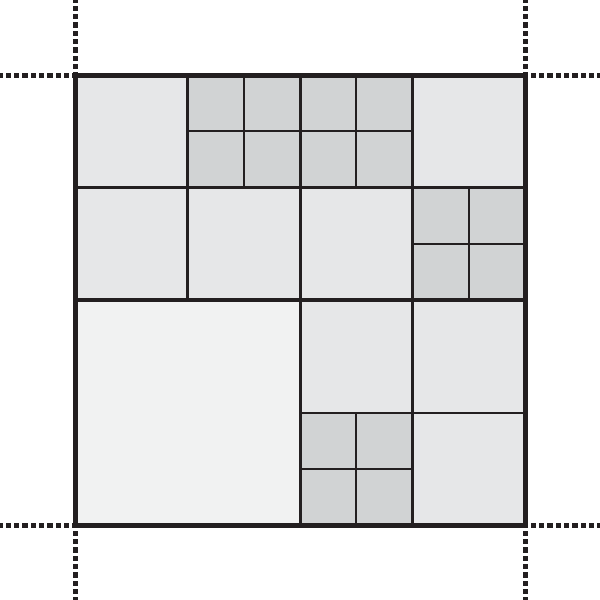
\includegraphics[width=0.4\textwidth]{quadtree1}
	\captionsetup{width=0.8\textwidth}
	\caption{Eksempel på udsnit af en quadtree-struktur hvori dybden af de individuelle quads fremhæves af disses farve, fra lys til mørk.}
	\label{fig:quadtree1}
\end{figure}
Når et rektangulært område efterspørges, foregår dette ligeledes rekursivt. En quad, som modtager en forespørgsel, vil videregive forespørgelsen til sine børn, og derefter returnere det tilbagemeldte resultat sammenlagt med sine egne elementer.

Det vurderes at en sorteret liste ville være for langsom til vores behov. Det var svært at sætte fingeren på en konkret forskel i ydeevnen mellem k-d-træet og quadtree-strukturen. Grundet et langt større kendskab til quadtree-strukturens virkemåde, sås denne således som den mest passende løsning. Vi fandt det vigtigt at vælge og udarbejde datastrukturen hurtigt, da udviklingen af resten af programmet afhang deraf.

\subsection{Linjeplacering}
Da en quadtree-struktur arbejder med et koordinatrum ved indsættelse og forespørgsel af data, er det nødvendigt at skabe en sammenhæng mellem et vejsegment og koordinatsystemet. Indledningsvist løste vi dette problem med blot at styre indsættelsen af en linje efter dens centrum. (\ref{fig:quadtree2} tv.). Dette forårsagede dog et større problem, hvor relativt lange linger ikke blev tegnet, da disses centrum kunne være uden for den besøgte quad. Vores umiddelbare løsning til dette var, at udvide den forespurgte rektangel den halve længde af den længste linje i den adspurgte quad. Således var det garanteret, at samtlige linjer, som skar det efterspurgte rektangel, faktisk blev fundet.
\begin{figure}[ht]
	\centering
	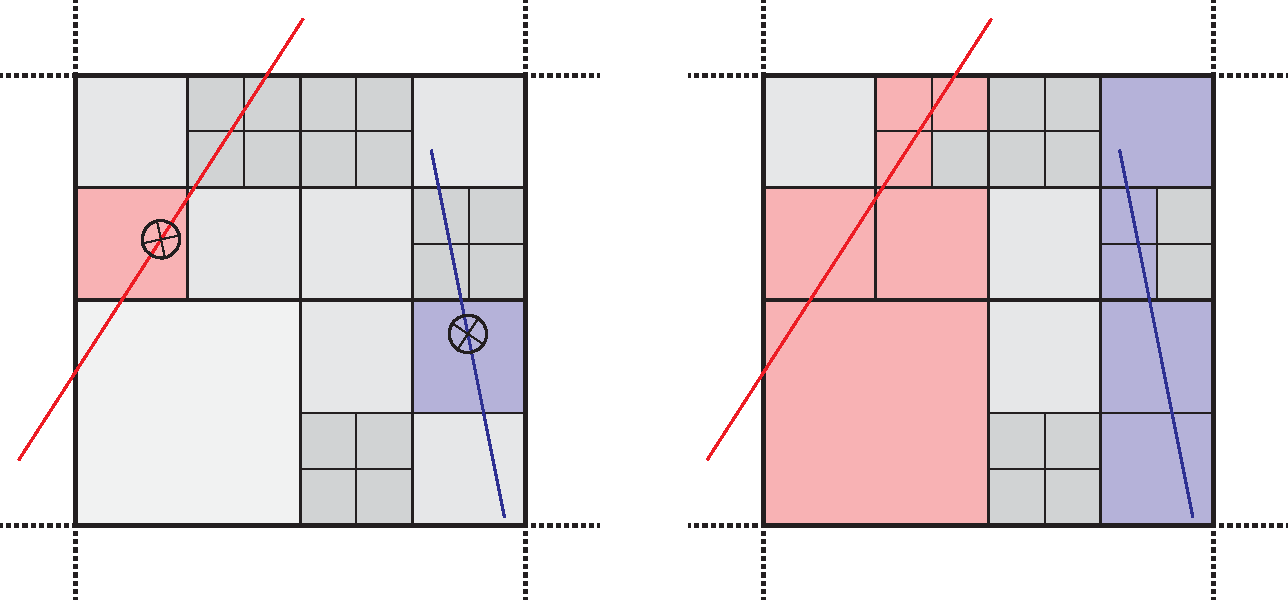
\includegraphics[width=0.7\textwidth]{quadtree2}
	\captionsetup{width=0.8\textwidth}
	\caption{Venstre: Linjens centrum afgør hvilken quad den placeres i. Højre: Linjen placeres i enhver quad, som denne skærer.}
	\label{fig:quadtree2}
\end{figure}
Denne implementering medførte, at andre dele af programmet, som gjorde brug af quadtree-strukturen, måtte regne med at modtage vejstykker uden for det forespurgte rektangel. Det ville senere vise sig at udgøre et reelt problem for programmets hastighed under tegneprocessen. Derfor ændrede vi måden hvorpå linjer indsættes i træet til en mere ideel tilgang, hvor enhver quad som berøres af en linje, indeholder denne. (\ref{fig:quadtree2} th.). Indhentning af et dataområde er således garanteret at returnere de linjer, som enten ligger indenfor eller skærer det eftersøgte område --- og intet andet.

\subsection{Nærmeste vej}
For at opfylde det formelle krav om at synliggøre navnet på vejen nærmest markøren, samt at muliggøre angivelse af udgangspunktet             og destinationen for navigation med markøren, måtte en algoritme udarbejdes. Udfordringen bestod i at gennemsøge quadtree-strukturen i et begrænset område omkring markøren. Hertil opstod et løsningsforslag, i at finde den dybeste quad, som markøren holdes over, og iterere over dennes indhold. Det medførte dog et problem, når markøren befandt sig tæt på en quads horisont, fordi det da ikke kunne garanteres, at den nærmeste vej befandt sig i den fundne quad. I stedet for at løse dette, ved at implementere en måde hvorpå nabo-quads kunne findes, valgte vi at udnytte allerede eksisterende funktionalitet til at løse det oprindelige problem. Ved at forespørge den øverste quad om vejstykker i en begrænset rektangel uden om markøren, og derefter gennemløbe resultatet, kunne det nærmeste vejstykke hurtigt findes. Fandt en forespørgsel ikke nogen vejstykker fordobledes det forespurgte rektangel, og der forsøgtes igen. Ved at fordoble søgearealet sænkes antallet af nødvendige iterationer, uanset om markøren er meget langt væk fra fastlandet eller midt i hovedstaden.
\begin{figure}[ht]
	\centering
	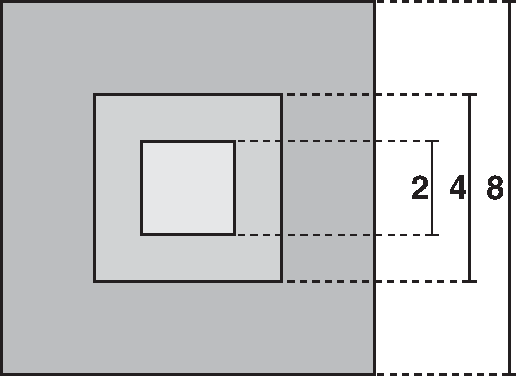
\includegraphics[width=0.5\textwidth]{naermestvej}
	\captionsetup{width=0.8\textwidth}
	\caption{Søgerektanglet fordobles for hver iteration, indtil mindst én linje er fundet.}
	\label{fig:naermestvej}
\end{figure}